\documentclass[conference]{IEEEtran}
\renewcommand{\ttdefault}{cmtt}
\addtolength{\topmargin}{0.06in}
\addtolength{\textheight}{-0.06in}

\usepackage{cite}
\usepackage{url}
\usepackage{amsmath,amssymb,amsfonts}
\usepackage{graphicx}
\usepackage{textcomp}
\usepackage{xcolor}
\def\BibTeX{{\rm B\kern-.05em{\sc i\kern-.025em b}\kern-.08em
    T\kern-.1667em\lower.7ex\hbox{E}\kern-.125emX}}

\begin{document}

\title{Regime-Dependent Utility of Open-Weight Large Language Models for Tabular Anomaly Detection}

\author{\IEEEauthorblockN{1\textsuperscript{st} Soumitra Mehrotra}
\IEEEauthorblockA{\textit{Independent Researcher}\\
San Francisco, CA, USA \\
soumitra.mehrotra9@gmail.com}
\and
\IEEEauthorblockN{2\textsuperscript{nd} Saurabh Aggarwal}
\IEEEauthorblockA{\textit{Independent Researcher}\\
San Francisco, CA, USA \\
sorav77@gmail.com}
}

\maketitle

\begin{abstract}
Tabular anomaly detection underpins fraud monitoring and intrusion detection.
Recent work reports that compact open-weight large language models (LLMs) can be competitive on benchmark AUROC, while other studies find LLMs underperform classical detectors.
We conducted a controlled replication and extension of AnoLLM, a recent likelihood-based method.
We reproduced SmolLM-360M likelihood scoring on the 30-dataset ODDS anomaly-detection benchmark suite, then compared likelihood scoring (base model with LoRA fine-tuning) against prompted scoring (frozen instruction-tuned model) for matched SmolLM-360M and Qwen2.5-3B models.
We further evaluated credit-card fraud and network-intrusion data (UNSW-NB15) under a fixed 1\% false-positive-rate (FPR) alert budget, along with several additional ablations.
The replication passed the two pre-registered aggregate gates (mean AUROC 0.851 vs.\ 0.865 published; rank correlation 0.875) but failed the stricter per-dataset band gate (19 of 30 datasets, threshold 24).
On ODDS, likelihood scoring outperformed the zero-shot expected-value prompted baseline (Friedman omnibus, p less than 1e-11); a stronger few-shot prompted baseline closed most of that gap (mean AUROC 0.759 vs.\ 0.773 for likelihood, difference not significant, Wilcoxon p=0.64 on eight datasets), so the advantage is specific to the zero-shot instantiation. The larger Qwen2.5-3B model did not significantly outperform SmolLM-360M under likelihood scoring.
At the 1\% FPR budget the two security datasets diverged: on credit-card fraud classical detectors far outperformed the tested LLM configurations (KNN 0.715 vs.\ 0.136 for Qwen2.5-3B likelihood), whereas on UNSW-NB15 Qwen2.5-3B likelihood scoring (recall@1\%FPR 0.302) exceeded every classical detector (best KNN 0.189).
Domain-informed column ordering and two-stage triage did not improve results.
Open-weight LLM likelihood scoring remains competitive at the aggregate benchmark level; under fixed-alert-budget conditions its standing was dataset-dependent, trailing classical detectors on credit-card fraud but leading them on UNSW-NB15 (two datasets; no cross-dataset claim).
Practitioners should not treat ODDS-style AUROC as a proxy for deployment-threshold recall.
\end{abstract}

\begin{IEEEkeywords}
Anomaly detection, large language models, replication studies, security analytics, tabular data
\end{IEEEkeywords}

\section{Introduction}\label{sec:intro}
Tabular anomaly detection supports fraud monitoring and intrusion detection.
Classical detectors such as Isolation Forest (IForest), $k$-nearest neighbors ($k$NN), and ECOD remain strong, low-cost baselines~\cite{zhao2019pyod,han2022adbench}.

Recent work asks whether large language models (LLMs) can detect anomalies from serialized tabular rows.
AnoLLM~\cite{tsai2025anollm} showed that small open models scoring rows by likelihood are competitive on ODDS, a standard suite of 30 tabular anomaly-detection benchmark datasets, under AUROC, while AD-LLM~\cite{yang2025adllm} reports that contemporary LLMs can underperform classical methods in NLP anomaly-detection settings, a different task domain.

The field therefore faces a precise, unresolved question: under what operating regime---model scale, scoring mode, data semantics, imbalance, and alert budget---do open-weight LLMs help for tabular anomaly detection, and where do classical detectors still dominate?
These conflicting findings suggest that LLM utility may depend less on model family alone than on the scoring rule, benchmark, and operating metric.

We study this question through a replication and extension of AnoLLM rather than by proposing a new detector.
Our study holds model family and size fixed while comparing two scoring modes: (A)~base model plus Low-Rank Adaptation (LoRA) fine-tuned likelihood scoring versus (B)~a frozen instruction-tuned sibling scored by prompted expected value.
We pre-registered replication gates before generating results, then extended evaluation to two security-relevant datasets with fixed-false-positive-rate (FPR) operational metrics, serialization ablations, and a two-stage triage design.

Our contributions are threefold.
First, we provide a controlled same-family, same-size likelihood-versus-prompted A/B on open-weight models (SmolLM-360M and Qwen2.5-3B); the base-versus-instruct checkpoint difference between the two modes is bounded empirically in Section~\ref{sec:method} (mean $|\Delta\mathrm{AUROC}|=0.0054$).
Second, we re-evaluate under realistic operating conditions on credit-card fraud and UNSW-NB15 using recall@1\%FPR, plus semantic-name and serialization-order ablations.
Third, we report three negative findings: the tested domain-informed column ordering did not help on pima and UNSW-NB15; semantic column names did not reliably help on pima ($n=3$ pairs, exploratory); and IForest-plus-LLM triage added zero uplift at $k=1\%$.

The security experiments rest on two datasets and are reported as per-dataset evidence only.
ODDS results use AUROC; security results use recall@1\%FPR.
The resulting evidence should therefore be interpreted as a replication and evaluation study rather than as a new detector proposal.
Overall, the results support a regime-dependent interpretation: likelihood scoring remains competitive under ODDS AUROC, while for fixed-FPR alerting the two security-relevant datasets diverge (classical ahead on credit-card fraud, LLM likelihood ahead on UNSW-NB15).
By \emph{regime-dependent} we mean that whether LLM scoring helps is determined jointly by the scoring mode, evaluation metric, and data regime (imbalance and alert budget), not by model family or size alone.
Table~\ref{tab:regime} summarizes the evaluation regimes and supported claims; every row is scoped to the datasets, metrics, and methods actually tested.
The remainder of this paper reviews related work (Section~\ref{sec:related}), describes the experimental method (Section~\ref{sec:method}), reports replication, scoring-mode, security-transfer, and ablation results (Section~\ref{sec:results}), discusses implications, limitations, and future directions (Section~\ref{sec:discussion}), and concludes (Section~\ref{sec:conclusion}).

\begin{table*}[t]
\caption{Summary of Evaluation Regimes and Supported Claims}
\label{tab:regime}
\begin{center}
\renewcommand{\arraystretch}{1.2}
\small
\begin{tabular}{|p{1.5in}|p{1.1in}|p{3.6in}|}
\hline
\textbf{Regime} & \textbf{Metric} & \textbf{Finding (tested methods)} \\
\hline
ODDS (30 datasets) & AUROC & Likelihood competitive at aggregate level; prompted expected-value baseline underperforms \\
ODDS (30 datasets) & AUROC & No significant difference between SmolLM-360M and Qwen2.5-3B under likelihood scoring \\
Credit-card fraud & Recall@1\%FPR & Classical detectors far outperform all tested LLM configurations (Qwen likelihood 0.136 vs.\ KNN 0.715) \\
UNSW-NB15 & Recall@1\%FPR & Qwen likelihood scoring (0.302) exceeds every classical detector (best 0.189); prompted scoring trails \\
Ablations & AUROC & Domain ordering: null on pima and UNSW-NB15; semantic names: null on pima only \\
Triage & Recall@FPR uplift & Zero uplift at $k$=1\%; harmful at wider $k$ \\
\hline
\end{tabular}
\end{center}
\end{table*}

\section{Related Work}\label{sec:related}
\textbf{LLMs for tabular anomaly detection.}
AnoLLM~\cite{tsai2025anollm} fine-tunes SmolLM models and scores rows by mean negative log-likelihood over random column permutations, reporting competitiveness with classical detectors on ODDS under AUROC.
It does not run a same-family likelihood-versus-prompted comparison, does not sweep open-weight scale for prompted scoring, and evaluates primarily by AUROC rather than fixed-FPR metrics.
AnoLLM's mixed-type evaluation includes two fraud-related datasets (fraud-ecommerce, vehicle-insurance) at 6--9\% anomaly rates; our security evaluation targets a substantially more imbalanced regime (0.17\% on credit-card fraud) using fixed-FPR metrics not reported in the original study.
Li et al.~\cite{li2024tabularllm} study \emph{batch-level} tabular anomaly detection, where the model sees a batch of rows and identifies the outlier row; they report GPT-4 competitive with state-of-the-art transductive methods on ODDS. Our work differs in three ways: scoring is \emph{per-row} (not batch-level), models are open-weight (not GPT-4), and we run a controlled A/B comparing likelihood to prompted scoring.
AD-LLM~\cite{yang2025adllm} benchmarks LLMs for anomaly detection in NLP settings (zero-shot text detection, data augmentation, model selection); it does not study tabular anomaly detection directly. Its findings motivate our regime-dependent framing, although it is not a direct tabular benchmark.

\textbf{Tabular serialization and generative tabular models.}
GReaT~\cite{borisov2023great} and TabLLM~\cite{hegselmann2023tabllm} serialize rows to text for generation or classification.
We reuse row serialization but study anomaly \emph{scoring} and treat column order as an explicit variable. CausalTAD~\cite{causaltad2026} proposes causal column ordering (modeled as a linear ordering problem) plus causal-aware column reweighting, arguing that causal structure between columns affects likelihood. Our serialization-order ablation addresses a strictly narrower question: whether a \emph{manually defined domain-informed order} improves prompted scoring. We do not test causal discovery, causal ordering derived from data, or column reweighting; a null result there does not address CausalTAD's causal reweighting mechanism.

\textbf{Benchmarks and classical baselines.}
ADBench~\cite{han2022adbench} and the ODDS library standardize datasets and baseline panels.
We adopt IForest, PCA, $k$NN, and ECOD from PyOD~\cite{zhao2019pyod} for comparability with AnoLLM's classical panel.
To our knowledge, no prior work jointly provides (i)~a controlled same-family, same-size open-weight likelihood-versus-prompted A/B with an empirical checkpoint bound, (ii)~fixed-FPR evaluation on two security-relevant datasets, and (iii)~a reported negative two-stage triage result.
These distinctions position the paper as a replication and evaluation extension rather than a new detection method.

\section{Method}\label{sec:method}

\subsection{Row Serialization}
Let a row $x$ have $d$ columns with names $(c_1,\ldots,c_d)$ and values $(v_1,\ldots,v_d)$.
Each row was rendered as \texttt{col is value, col is value, \ldots} following AnoLLM.
Numerical preprocessing on ODDS followed AnoLLM's ``standard'' protocol; the same transformation was applied consistently across likelihood and prompted comparisons.
Security loaders returned raw floats; this protocol difference is documented and bounded by a binned credit-card check (BA1).
The same serialization was shared across both scoring modes within each comparison.
Column order was fixed within a comparison and varied only in the serialization-order ablation.

\subsection{Scoring Modes}
\textbf{Mode A (likelihood).}
The base model (SmolLM-360M or Qwen2.5-3B) was fine-tuned with LoRA~\cite{hu2022lora} on normal training rows.
For a test row $x$ and permutation $r$, let $T_r(x)$ denote the token positions corresponding to serialized field values (column-name tokens excluded).
The anomaly score was
\begin{equation}
s(x)=\frac{1}{R}\sum_{r=1}^{R}\frac{1}{|T_r(x)|}\sum_{t\in T_r(x)}-\log p_\theta(y_t \mid y_{<t}),
\end{equation}
averaged over $R=10$ random column permutations, with per-column length normalization for textual fields.

\textbf{Mode B (prompted).}
The frozen instruction-tuned sibling (SmolLM-360M-Instruct or Qwen2.5-3B-Instruct) read the serialized row.
Prompts used the form: ``Record: [serialized row]. How anomalous is this record on a scale of 0 (normal) to 9 (highly anomalous)? Answer with a single digit.''
We computed a continuous score as the expected value over anomaly-level digit tokens from a single forward pass.
This expected-value scoring is one specific instantiation of prompted anomaly detection.
The main A/B uses this zero-shot instantiation; we separately evaluate a normals-only few-shot variant (Section~\ref{subsec:scoringmode}). We do not evaluate chain-of-thought, pairwise, or calibrated temperature-scaled variants. Conclusions on the zero-shot Mode B baseline apply to that instantiation only and should not be taken as the final word on all prompting methods.

\textbf{Model choice and scale range.}
SmolLM-360M~\cite{allal2024smollm} was chosen to match AnoLLM's backbone for the replication.
Qwen2.5-3B~\cite{qwen2025qwen25} was chosen as an open-weight model at an 8$\times$ larger scale feasible within the same hardware budget. The study is limited to the 360M--3B parameter range; results may not hold for 7B-scale models, different architectures, or instruction-tuned checkpoints outside the tested SmolLM-360M and Qwen2.5-3B families.

Mode A uses a base+LoRA checkpoint and Mode B uses a frozen instruct checkpoint, so the two modes differ in both scoring method and checkpoint.
A checkpoint-confound control (DA1) LoRA-fine-tuned Qwen2.5-3B-Instruct and scored by likelihood on eight ODDS datasets, comparing against the corresponding Qwen2.5-3B base+LoRA cells, to bound this confound.

\subsection{Metrics and Statistics}
AUROC (tie-aware) was used for ODDS comparability; it measures ranking quality across all score thresholds and does not specify performance at a single alert budget.
On security data we reported recall@1\%FPR as the primary metric and area under the precision-recall curve (AUPRC) relative to prevalence with importance reweighting after negative subsampling as a secondary imbalance-aware view.
Recall@1\%FPR is the recall at the ROC operating point $\tau^*$ with the largest false-positive rate not exceeding 1\%, computed from scikit-learn's ROC curve (ties grouped at shared thresholds).
\begin{equation}
\text{Recall@1\%FPR}=\mathrm{TPR}(\tau^*).
\end{equation}
Recall@1\%FPR is the primary security metric because operational fraud and intrusion-detection systems typically work at a fixed alert budget: only the top-$k$ ranked cases are investigated.
ODDS ($n=30$ datasets): Friedman omnibus, Nemenyi critical-difference diagram, and Holm-corrected Wilcoxon signed-rank for pre-registered pairwise claims.
Security ($n=2$ datasets): per-dataset mean $\pm$ std over 3 seeds; no Friedman test.

\subsection{Experimental Controls}
Replication gates (C1--C3), confound checks (DA1, BA1), experiment grids, AnoLLM reference targets, and mode-specific hyperparameters were fixed before result generation.
Prompt templates for Mode B were held constant across runs.
Each completed cell recorded seeds, train/test splits, hyperparameters, and metrics in standardized run metadata.
Likelihood runs used SmolLM-360M at 2000 training steps and Qwen2.5-3B at 1000 steps, with $R=10$ random column permutations and LoRA fine-tuning via the Parameter-Efficient Fine-Tuning (PEFT) library.
Dependencies were pinned to \texttt{torch==2.3.1} and \texttt{transformers==4.48.2}.
We do not claim bit-exact reproduction of AnoLLM's published fork; the per-dataset shortfall is reported in the replication results.

\subsection{Protocol Checks}
\textbf{DA1 (checkpoint-confound control).} Instruct-checkpoint likelihood yielded mean $|\Delta\mathrm{AUROC}|=0.0054$ vs.\ base+LoRA across eight ODDS datasets (threshold 0.02).
\textbf{BA1 (binned credit-card).} Switching credit-card from raw floats to ODDS-style binning changed mean classical AUROC by 0.0012 across four detectors (threshold 0.03).
\textbf{T3 (Time feature).} On temporal credit-card splits, including the \texttt{Time} column collapsed $k$NN AUROC from 0.932 to 0.178.
The \texttt{Time} column encodes absolute transaction order; including it introduces a non-stationarity artifact that can dominate distance-based scores, so all reported classical credit-card results use the time-excluded protocol.

\section{Results}\label{sec:results}

\subsection{Replication}\label{subsec:replication}
SmolLM-360M likelihood scoring passed the two pre-registered aggregate gates (C1, C2) but failed the stricter per-dataset band gate (C3).
Mean AUROC was 0.851 vs.\ AnoLLM's reported 0.865 ($\Delta=0.0145$, C1 pass).
Spearman rank correlation across 30 datasets was $\rho=0.875$ (C2 pass).
Nineteen of 30 datasets fell within the pre-registered per-dataset band (C3 threshold 24/30, fail).
The eleven out-of-band datasets were cardio, covertype, ecoli, letter, optdigits, pendigits, satellite, vowels, wbc, wine, and yeast; the deviations were bidirectional (our mean AUROC exceeded the reference on cardio, covertype, ecoli, wine, and yeast but fell short on letter, optdigits, pendigits, satellite, vowels, and wbc), so the shortfall is not a uniform downward bias.
Under the pre-registered decision rule, C1 and C2 were the hard-stop criteria; the replication is a credible partial reproduction.
These checks did not identify a protocol error; candidate explanations consistent with our controls are (i) the released AnoLLM fork differing from the published configuration---a grad-accumulation (effective-batch) test moved letter and satellite by only 0.02--0.03 AUROC, insufficient to close the gap---and (ii) LoRA fine-tuning instability on small tabular datasets.

\subsection{Scoring Mode}\label{subsec:scoringmode}
Likelihood scoring outperformed the zero-shot expected-value prompted baseline across 360 cells (30 ODDS datasets $\times$ 4 conditions (2 models $\times$ 2 modes) $\times$ 3 seeds).
The Friedman omnibus test rejected equal performance ($\chi^2_F=55.27$, $p=6.0\times10^{-12}$, $k=4$, $n=30$).
Average ranks (lower is better): SmolLM-likelihood 1.62, Qwen-likelihood 1.65, SmolLM-prompted 3.20, Qwen-prompted 3.53.
A likelihood condition ranked first on 28 of 30 datasets; both prompted conditions ranked third or fourth on 28 of 30.
Holm-corrected Wilcoxon tests against SmolLM-likelihood: both prompted conditions were significantly worse (SmolLM-prompted: median $\Delta=-0.276$, $p_{\mathrm{Holm}}=1.4\times10^{-7}$; Qwen-prompted: median $\Delta=-0.339$, $p_{\mathrm{Holm}}=9.4\times10^{-7}$).
Thus, for ODDS-style AUROC, likelihood scoring outperforms the zero-shot expected-value prompted baseline in our experiments.

To test whether this advantage reflects the weakness of the zero-shot baseline rather than an intrinsic likelihood benefit (reviewer concern), we evaluated a stronger prompted baseline that prepends three normal exemplars (normals-only few-shot) on eight ODDS datasets with Qwen2.5-3B-Instruct.
Few-shot prompting raised mean AUROC from 0.468 (zero-shot) to 0.759, closing about 95\% of the gap to likelihood scoring (0.773 on the same eight datasets).
The residual 0.014 difference was not statistically significant (paired Wilcoxon on eight dataset means, $p=0.64$, $n=8$). At $n=8$ the minimum achievable Wilcoxon $p$ is ${\approx}0.008$; the non-significant result therefore indicates the two modes are statistically indistinguishable at the available power, not that they are provably equal.
Gains were not uniform: few-shot helped substantially on breastw, yeast, and ionosphere but regressed on speech and vertebral.
We therefore narrow the scoring-mode claim: likelihood scoring outperforms the \emph{zero-shot} expected-value baseline used in the main A/B, but is statistically indistinguishable from a few-shot prompted baseline on these eight datasets.

Table~\ref{tab:rq2} summarizes condition means.
Fig.~\ref{fig:cd} shows the critical-difference diagram, where the two likelihood conditions form a cluster distinct from both prompted conditions.
The replication run (max\_steps=2000) reports SmolLM-360M AUROC 0.851; the scoring-mode comparison uses independently initialized runs, giving 0.843 for the same model and mode.
The difference (0.008) reflects run-to-run variance across independently seeded training runs; the C1 replication gate (Section~\ref{subsec:replication}) is evaluated on the pre-registered replication run (0.851) and is not affected by this later, independently seeded comparison.

\begin{table}[htbp]
\caption{ODDS Mean AUROC and Average Rank by Condition ($n=30$ Datasets, 3 Seeds)}
\label{tab:rq2}
\begin{center}
\renewcommand{\arraystretch}{1.2}
\begin{tabular}{|l|c|c|}
\hline
\textbf{Condition} & \textbf{Mean AUROC} & \textbf{Avg.\ rank} \\
\hline
SmolLM-360M / likelihood & 0.843 & 1.62 \\
Qwen2.5-3B / likelihood   & 0.859 & 1.65 \\
SmolLM-360M / prompted    & 0.610 & 3.20 \\
Qwen2.5-3B / prompted     & 0.493 & 3.53 \\
\hline
\end{tabular}
\end{center}
\end{table}

\begin{figure}[htbp]
\centerline{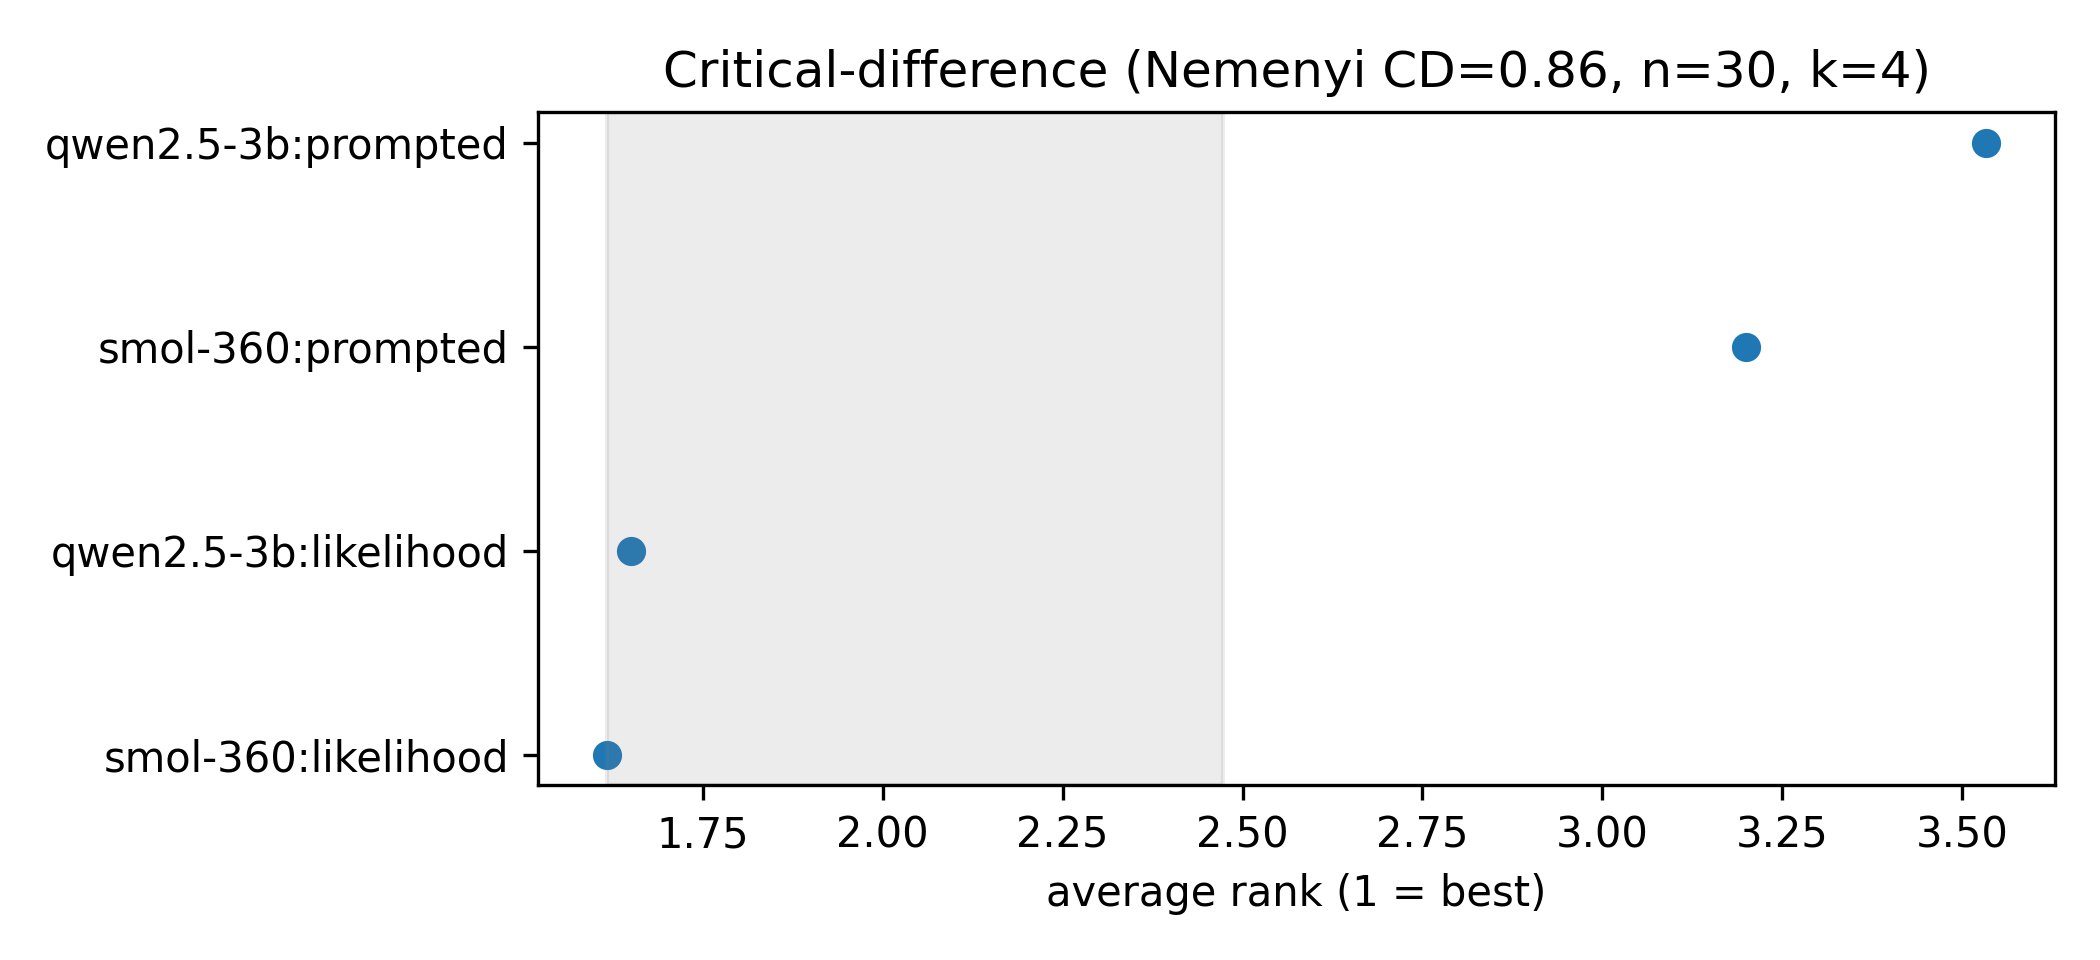
\includegraphics[width=\columnwidth]{figures/fig_cd.png}}
\caption{Critical-difference diagram for four conditions on 30 ODDS datasets (Friedman $p=6.0\times10^{-12}$). Connected conditions are not significantly different by Nemenyi post-hoc test.}
\label{fig:cd}
\end{figure}

\subsection{Model Scale}
Within likelihood scoring, Qwen2.5-3B (mean AUROC 0.859) did not significantly outperform SmolLM-360M (0.843; Holm-corrected Wilcoxon $p=0.77$).
This is consistent with AnoLLM's finding that larger models do not improve NLL-based anomaly scoring on predominantly numerical ODDS data.
Scale upgrades within the tested open-weight range do not justify the added compute for likelihood scoring on ODDS.
This null on scale is bounded to the 360M--3B range tested here; we did not evaluate 7B+ models, which many open-weight practitioners deploy, so the scale claim should not be extrapolated beyond this range.

\subsection{Semantic Column Names}
On pima, replacing integer column indices with descriptive names changed mean AUROC by $-0.007\pm0.021$ across three seed pairs (individual deltas: $+0.016$, $-0.026$, $-0.010$).
This is a null result at $n=3$ pairs (minimum achievable Wilcoxon $p=0.25$); we report descriptive evidence only.
Semantic column names did not reliably improve prompted or likelihood scoring at this granularity.

\subsection{Fixed-FPR Security Evaluation}
At the 1\% FPR operating point the two security datasets diverged (Table~\ref{tab:rq4}): classical detectors dominated on credit-card fraud, whereas Qwen2.5-3B likelihood scoring led all classical detectors on UNSW-NB15.
Table~\ref{tab:rq4} reports recall@1\%FPR (mean $\pm$ std over 3 seeds).
Likelihood scoring (mode A) was run on credit-card fraud (6 cells: 2 splits $\times$ 3 seeds) and, in this revision, on UNSW-NB15 (3 seeds; this arm was previously omitted to bound GPU cost).
SmolLM-360M likelihood scoring was not included in the pre-specified security grid; the likelihood arm targets Qwen2.5-3B only, consistent with the pre-registered design.
On credit-card fraud (random split, time excluded), KNN achieved 0.715$\pm$0.015, ECOD 0.680$\pm$0.003, and IForest 0.586$\pm$0.029, while Qwen likelihood reached 0.136$\pm$0.017 and Qwen prompted 0.003$\pm$0.001.
On UNSW-NB15, Qwen2.5-3B likelihood scoring reached recall@1\%FPR 0.302$\pm$0.026, exceeding the leading classical detectors (KNN 0.189$\pm$0.012, IForest 0.188$\pm$0.018) and the prompted baseline (0.151$\pm$0.013).
The ordering thus reversed between datasets: classical far ahead on credit-card fraud, LLM likelihood ahead on UNSW-NB15.
On the secondary AUPRC-gain view the UNSW ordering was mixed (ECOD 9.3, IForest 9.2, Qwen likelihood 7.7, PCA 7.6, KNN 5.8), so the LLM advantage on UNSW is specific to recall@1\%FPR; on credit-card fraud classical AUPRC-gain far exceeded LLMs (ECOD 88$\times$, IForest 66$\times$, PCA 76$\times$, KNN 59$\times$ vs.\ Qwen likelihood 7$\times$).
Fig.~\ref{fig:security} plots recall@1\%FPR by method on both datasets: classical detectors cluster well above both Qwen configurations on credit-card fraud, while Qwen likelihood is the top bar on UNSW-NB15.
AUROC alone is misleading in these settings: IForest AUROC was 0.951 on the credit-card random split, but recall@1\%FPR was 0.586 vs.\ 0.136 for Qwen likelihood; ECOD AUROC was 0.950 yet recall@1\%FPR was 0.680.
Section~\ref{subsec:triage} examines whether two-stage re-ranking closes this gap.

\begin{table}[htbp]
\caption{Recall@1\%FPR on Two Security-Relevant Datasets (Mean $\pm$ Std, 3 Seeds). Credit-card uses time-excluded protocol. Qwen likelihood is now evaluated on both datasets; on UNSW-NB15 it leads all classical detectors.}
\label{tab:rq4}
\begin{center}
\renewcommand{\arraystretch}{1.2}
\small
\begin{tabular}{|l|c|c|}
\hline
\textbf{Method} & \textbf{CC (random)} & \textbf{UNSW-NB15} \\
\hline
KNN (classical)         & 0.715$\pm$0.015 & 0.189$\pm$0.012 \\
ECOD (classical)        & 0.680$\pm$0.003 & 0.161$\pm$0.006 \\
PCA (classical)         & 0.631$\pm$0.004 & 0.099$\pm$0.002 \\
IForest (classical)     & 0.586$\pm$0.029 & 0.188$\pm$0.018 \\
Qwen2.5-3B / likelihood & 0.136$\pm$0.017 & \textbf{0.302$\pm$0.026} \\
Qwen2.5-3B / prompted   & 0.003$\pm$0.001 & 0.151$\pm$0.013 \\
SmolLM-360M / prompted  & 0.011$\pm$0.004 & 0.009$\pm$0.001 \\
\hline
\end{tabular}
\end{center}
\end{table}

\begin{figure}[htbp]
\centerline{
\includegraphics[width=\columnwidth]{figures/fig_security.png}}
\caption{Recall@1\%FPR by method on credit-card fraud and UNSW-NB15.}
\label{fig:security}
\end{figure}

\subsection{Serialization Order}
The domain ordering for UNSW-NB15 placed network-level identification features (e.g., source/destination ports, protocol type) first, followed by traffic volume statistics, then payload features. For pima it followed demographic and clinical measurement fields in the dataset's conventional order. Both orderings were defined prior to running the experiment and held fixed across all seeds.
Mean AUROC by ordering condition (Qwen2.5-3B prompted, 3 seeds) is shown in Fig.~\ref{fig:ordering}.
Pooled across pima and UNSW-NB15: arbitrary 0.564, random-0 0.550, random-1 0.543, domain 0.501.
On pima (8 columns), arbitrary and domain orderings tied at 0.449 AUROC; random column shuffles achieved 0.526 and 0.553, indicating the fixed arbitrary ordering is suboptimal for this dataset.
On UNSW-NB15 (47 columns), arbitrary ordering (0.680) outperformed domain ordering (0.554) by 0.126 AUROC.
The tested domain-informed ordering did not improve LLM anomaly scoring on pima (tied with arbitrary at 0.449) and hurt performance on UNSW-NB15 relative to the default arbitrary ordering.
A single hand-designed ordering per dataset cannot rule out that some other informed ordering helps; we tested one domain ordering, not the space of informed orderings.

\begin{figure}[htbp]
\centerline{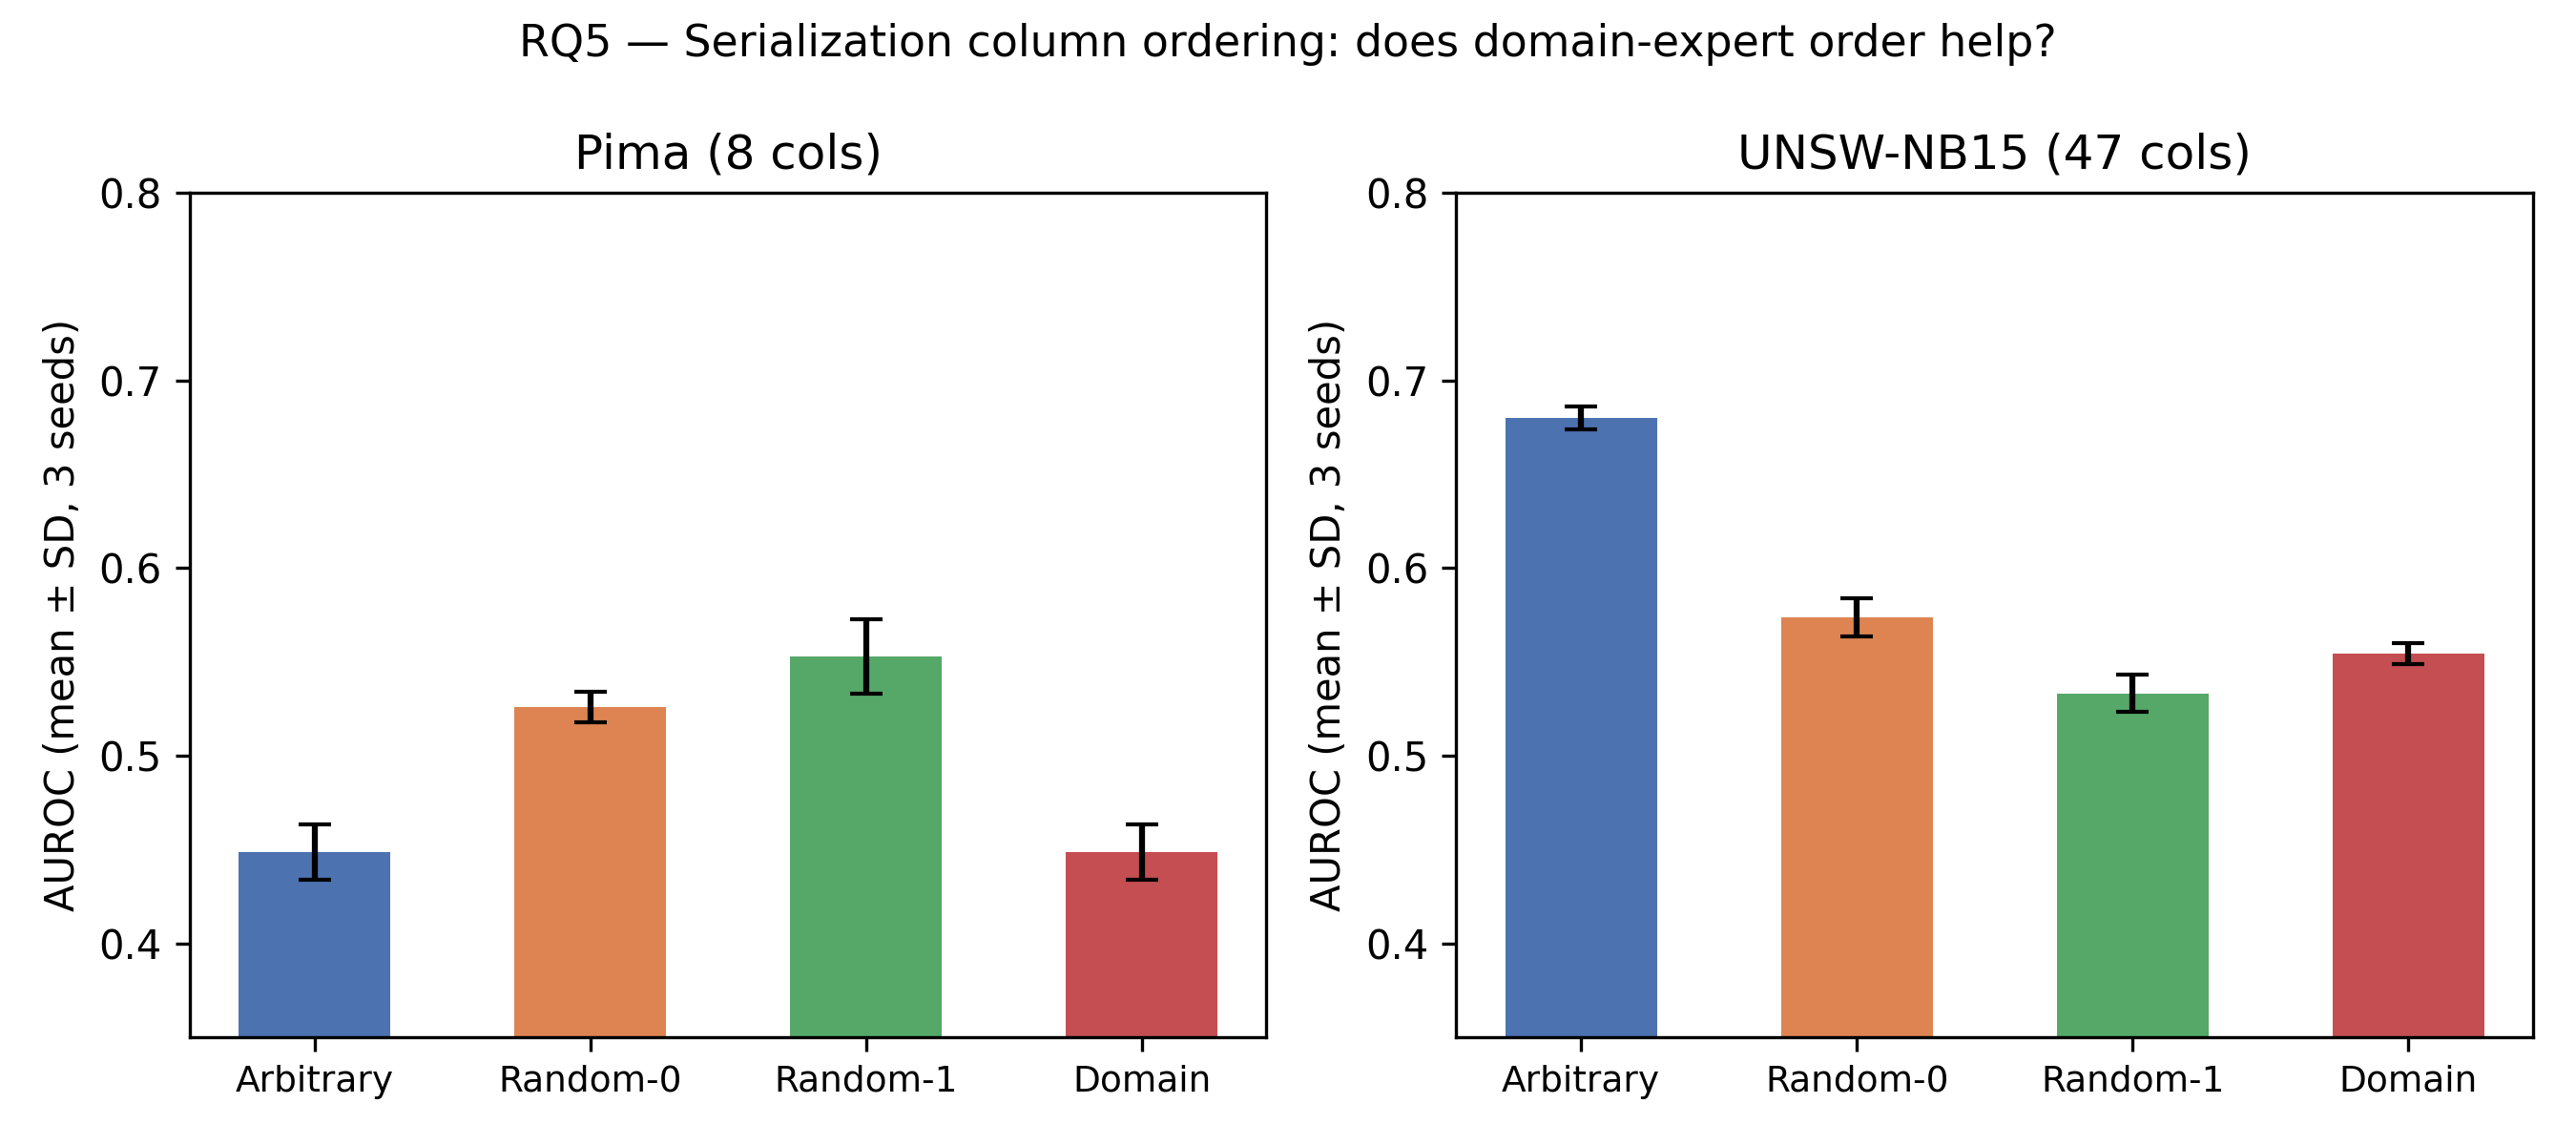
\includegraphics[width=\columnwidth]{figures/fig_ordering.png}}
\caption{Mean AUROC by serialization column ordering on pima and UNSW-NB15 (Qwen2.5-3B prompted, 3 seeds per condition).}
\label{fig:ordering}
\end{figure}

\subsection{Practicality}
Fig.~\ref{fig:pareto} plots mean AUROC against wall time per 1{,}000 test rows.
Timings were measured as elapsed runtime on NVIDIA A40 GPUs within the same hardware pool; they include LoRA fine-tuning and inference for Mode A, and inference only for Mode B, but not dataset download.
Qwen2.5-3B likelihood achieved mean AUROC 0.859 at ${\approx}$222\,s per 1{,}000 test rows (RUNLOG-approximated aggregate for the likelihood runs).
Qwen2.5-3B prompted achieved 0.493 at ${\approx}$33\,s per 1{,}000 test rows.
IForest runs in under 5\,s per 1{,}000 test rows with AUROC above 0.80 on ODDS.
The Pareto figure also shows a triage point (0.687 AUROC at ${\approx}$54\,s per 1{,}000 test rows); this is the LLM re-ranker component's AUROC evaluated in isolation, not the two-stage system AUROC.
The full triage system does not improve over IForest on the security-relevant datasets; its utility is evaluated by recall@FPR uplift in~Section~\ref{subsec:triage}.
Likelihood scoring offers higher AUROC at substantially higher cost than prompted scoring; in this implementation, IForest occupies a more favorable speed-accuracy region than the tested LLM scoring modes.

\begin{figure}[htbp]
\centerline{
\includegraphics[width=\columnwidth]{figures/fig_pareto.png}}
\caption{Mean AUROC vs.\ wall time per 1{,}000 test rows for tested LLM and classical scoring modes.}
\label{fig:pareto}
\end{figure}

\begin{table}[htbp]
\caption{Approximate Compute Cost per 1{,}000 Test Rows (NVIDIA A40). ODDS likelihood/prompted timings are RUNLOG-level approximations (flat per-mode constants); triage is measured per cell.}
\label{tab:compute}
\begin{center}
\renewcommand{\arraystretch}{1.2}
\begin{tabular}{|l|c|l|}
\hline
\textbf{Method} & \textbf{Wall (s/1k)} & \textbf{Source} \\
\hline
Qwen2.5-3B likelihood           & ${\approx}$222 & RUNLOG-approx \\
Qwen2.5-3B prompted (zero-shot) & ${\approx}$33  & RUNLOG-approx \\
LLM triage re-ranker            & ${\approx}$54  & measured \\
IForest (classical)             & $<$5           & approx \\
\hline
\end{tabular}
\end{center}
\end{table}

\subsection{Two-Stage Triage}\label{subsec:triage}
Two-stage triage re-ranks an IForest shortlist using Qwen2.5-3B prompted scoring; its effect is measured as an uplift in recall@$k$FPR relative to IForest alone:
\begin{equation}
\text{Uplift}(k)=\text{Recall@}k\text{FPR}_{\text{triage}}-\text{Recall@}k\text{FPR}_{\text{IForest}}.
\end{equation}
At $k=1\%$ (IForest shortlist then Qwen2.5-3B prompted re-rank), uplift in recall@1\%FPR was 0.00 across all nine cells (3 datasets $\times$ 3 seeds).
At $k=10\%$, the LLM re-ranker was harmful: mean uplift was $-0.489$ on credit-card random, $-0.455$ on credit-card temporal, and $-0.089$ on UNSW-NB15.
Table~\ref{tab:rq7} summarizes triage uplift.
At $k=1\%$, LLM re-ranking does not recover additional anomalies beyond the IForest shortlist; at wider shortlists, LLM re-ranking lowers recall relative to the original IForest ranking.

\begin{table}[htbp]
\caption{Two-Stage Triage Uplift in Recall@FPR (IForest + Qwen2.5-3B Prompted Re-Rank, Mean Over 3 Seeds). Negative values indicate LLM re-ranking degraded performance.$^{\mathrm{a}}$}
\label{tab:rq7}
\begin{center}
\renewcommand{\arraystretch}{1.2}
\begin{tabular}{|l|c|c|c|}
\hline
\textbf{Dataset} & \textbf{$k=1\%$} & \textbf{$k=5\%$} & \textbf{$k=10\%$} \\
\hline
Credit-card (random)   & 0.00 & $-0.330$ & $-0.489$ \\
Credit-card (temporal) & 0.00 & $-0.299$ & $-0.455$ \\
UNSW-NB15              & 0.00 & $-0.032$ & $-0.089$ \\
\hline
\end{tabular}
\par\smallskip\footnotesize $^{\mathrm{a}}$IForest baseline here (0.603) is from the triage experiment; Table~\ref{tab:rq4} reports 0.586 from an independent security experiment run. Seed variance accounts for the difference.
\end{center}
\end{table}

\section{Discussion}\label{sec:discussion}

\subsection{Interpretation}
The experimental sequence forms a cumulative argument. Replication establishes aggregate agreement with AnoLLM. The scoring-mode and model-scale comparisons show that likelihood scoring, rather than model scale, explains the ODDS result in the tested range. The fixed-FPR security evaluation shows that ODDS AUROC success does not imply deployment utility at fixed alert quotas. The serialization and triage ablations show that natural modifications---semantic names, manual domain-informed ordering, and hybrid triage---do not close the gap.

The ODDS experiments indicate that scoring mode matters more than model scale in the tested range.
A likelihood condition ranked first on 28 of 30 datasets; both prompted conditions ranked third or fourth on 28 of 30.
Prompted expected-value scoring collapses per-token probability into a single digit, discarding the distributional signal that likelihood scoring preserves.

The two security-relevant datasets pointed in opposite directions at fixed 1\% FPR.
On credit-card fraud, KNN, ECOD, and IForest delivered recall@1\%FPR of 0.715, 0.680, and 0.586 while Qwen likelihood reached 0.136 and Qwen prompted 0.003.
On UNSW-NB15, in contrast, Qwen likelihood scoring led all classical detectors on recall@1\%FPR (0.302 vs.\ KNN 0.189), reversing the credit-card ordering, though on the secondary AUPRC-gain view the UNSW ordering was mixed.
With two datasets that disagree, we draw no cross-dataset conclusion; the divergence itself reinforces that fixed-FPR utility is regime-dependent.
Practitioners operating at a fixed alert quota should evaluate recall at the alert threshold, not AUROC alone.

The tested serialization changes did not improve performance.
The tested domain-informed ordering did not help (pima tied at 0.449; UNSW arbitrary exceeded domain by 0.126 AUROC).
Semantic column names did not reliably help (mean $\Delta=-0.007$, $n=3$ pairs).

Two-stage triage does not close the fixed-FPR gap on the two security-relevant datasets.
At $k=1\%$, LLM re-ranking does not recover additional anomalies beyond the IForest shortlist; at wider $k$, re-ranking is harmful.

AnoLLM~\cite{tsai2025anollm} reports strong LLM performance under likelihood scoring on tabular ODDS benchmarks; Li et al.~\cite{li2024tabularllm} show GPT-4-level batch detection competitive with transductive methods on the same data; AD-LLM~\cite{yang2025adllm} finds variable LLM performance in NLP anomaly-detection settings. These results are mutually consistent once scoring mode (likelihood vs.\ prompted), evaluation metric (AUROC vs.\ recall@FPR), and data regime (benchmark numerical ODDS vs.\ extreme-imbalance security-relevant data) are stated explicitly.
AUROC-only comparisons can therefore be misleading for alert-budgeted deployments on imbalanced data.

\subsection{Limitations}
The C3 per-dataset band criterion failed (19/30 vs.\ threshold 24/30).
Timing estimates for likelihood and prompted modes are RUNLOG-level aggregate approximations, not per-cell wall clock.
Security results rest on two datasets that, at fixed 1\% FPR, point in opposite directions (classical best on credit-card fraud, Qwen likelihood best on UNSW-NB15); we therefore make no cross-dataset generalization claim.
The likelihood-versus-prompted A/B compares base+LoRA vs.\ frozen instruct; the checkpoint-confound control bounds but does not eliminate this confound.
Semantic-name and serialization-order ablations use $n=3$ seed pairs and are exploratory.
The few-shot-versus-likelihood comparison rests on $n=8$ dataset means (minimum achievable Wilcoxon $p\approx0.008$); its non-significant result is likewise underpowered rather than proof of equality.
We report implementation controls and run metadata sufficient to interpret the experiments, but do not claim artifact-level reproducibility beyond the protocol described here.

\subsection{Future Work}
A broader security benchmark (more than five datasets) would enable Friedman-powered cross-dataset tests, especially given that our two datasets disagree at fixed FPR.
LoRA fine-tuning stability on small tabular datasets warrants investigation given the C3 shortfall.
Higher-recall shortlisting stages and calibrated prompted scoring remain unexplored alternatives to the tested expected-value baseline.

\section{Conclusion}\label{sec:conclusion}
We presented a controlled replication and extension of AnoLLM for open-weight LLM-based tabular anomaly detection, holding model family and size fixed across likelihood and prompted scoring modes.
The evidence is regime-dependent: likelihood scoring remains competitive under aggregate ODDS AUROC, matching AnoLLM's published result on the two pre-registered aggregate gates (the per-dataset band gate failed), while at fixed alert budgets the two security-relevant datasets disagree (classical ahead on credit-card fraud, Qwen likelihood ahead on UNSW-NB15), and none of the tested modifications (semantic column names, domain-informed ordering, or two-stage triage) changed the ODDS picture.
Benchmark AUROC and deployment-relevant recall are not interchangeable; the choice between an LLM-based and a classical detector should be made against the metric and regime a system will actually operate under.

\section*{Acknowledgment}
The authors used ChatGPT for grammar, spelling, wording polish, and readability suggestions. ChatGPT was also used to assist in drafting Matplotlib Python plotting code from the authors' underlying data, calculations, and metrics. The reported results, analyses, and figures were generated and verified by the authors, who take full responsibility for the manuscript content.

\bibliographystyle{IEEEtran}
\bibliography{references}

\end{document}
